\documentclass[../main_proj4_correct_template.tex]{subfiles}

\graphicspath{{\subfix{Figures/}}}

\begin{document}


\section{Results and discussion}\label{sec:p4_results_and_discussion}

\subsection{Benchmarking against analytical values}

To benchmark the simulation algorithm, we use the analytical expressions from Section \ref{sec:p4_method_benchmark} and numerical simulations with a $2\times 2$ lattice. Further, we set $J=k_B=1$. Figures \ref{fig:p4_eps}, \ref{fig:p4_cv}, \ref{fig:p4_mabs} and \ref{fig:p4_chi} show the relation between $\mathbb{E}[\epsilon]$, $C_V/N$, $\mathbb{E}[|m|]$, $\chi/N$ and temperature, respectively. Here the blue line indicates the analytical values, while the red dots are the numerical values estimated after $10^{6}$ Monte-Carlo cycles.

\begin{figure}[h!]
    \centering
    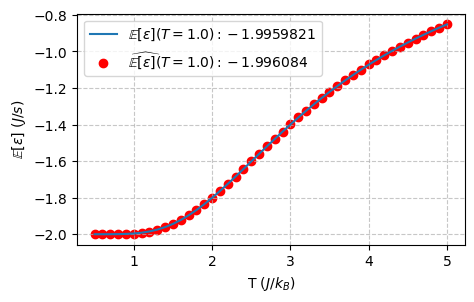
\includegraphics[width=0.8\linewidth]{Project 4/figures/p4_eps.png}
    \caption{The expectation value of the energy per dipole $\epsilon$ as a function of temperature $T$ for a $2\times 2$ Ising model. The analytical and numeric value at $T=1~J/k_B$ is shown in the legend.}
    \label{fig:p4_eps}
\end{figure}
\begin{figure}[h!]
    \centering
    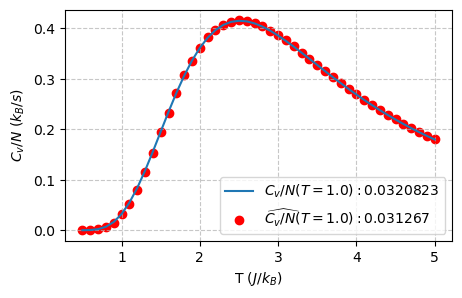
\includegraphics[width=0.8\linewidth]{Project 4/figures/p4_cv.png}
    \caption{The heat capacity per dipole $C_V/N$ as a function of temperature $T$ for a $2\times 2$ Ising model. The analytical and numeric value at $T=1~J/k_B$ is shown in the legend.}
    \label{fig:p4_cv}
\end{figure}
\begin{figure}[h!]
    \centering
    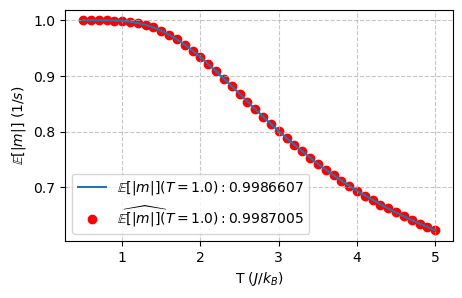
\includegraphics[width=0.8\linewidth]{Project 4/figures/p4_mabs.png}
    \caption{The expectation value of the absolute value of magnetization per dipole $|m|$ as a function of temperature $T$ for a $2\times 2$ Ising model. The analytical and numeric value at $T=1~J/k_B$ is shown in the legend.}
    \label{fig:p4_mabs}
\end{figure}
\begin{figure}[h!]
    \centering
    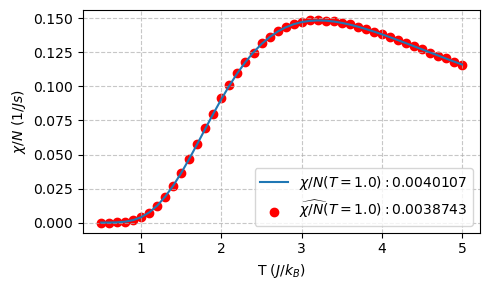
\includegraphics[width=0.8\linewidth]{Project 4/figures/p4_chi.png}
    \caption{The susceptibility per dipole $\chi/N$ as a function of temperature $T$ for a $2\times 2$ Ising model. The analytical and numeric value at $T=1~J/k_B$ is shown in the legend.}
    \label{fig:p4_chi}
\end{figure}

The figures show that there is a high degree of agreement between the numerical simulations and the analytical results. We choose to display the estimated value after $10^{6}$ cycles because the numerical value, in general, does not converge towards the analytical value before $10^{4}$ cycles for all variables. This is shown in Figure \ref{fig:p4_appB_p4_convergence}. However, since the lattice size is very small, we do not consider the physical implications of these results.

\subsection{Equilibration Cycle}

\begin{figure*}[htb!]
    \centering
    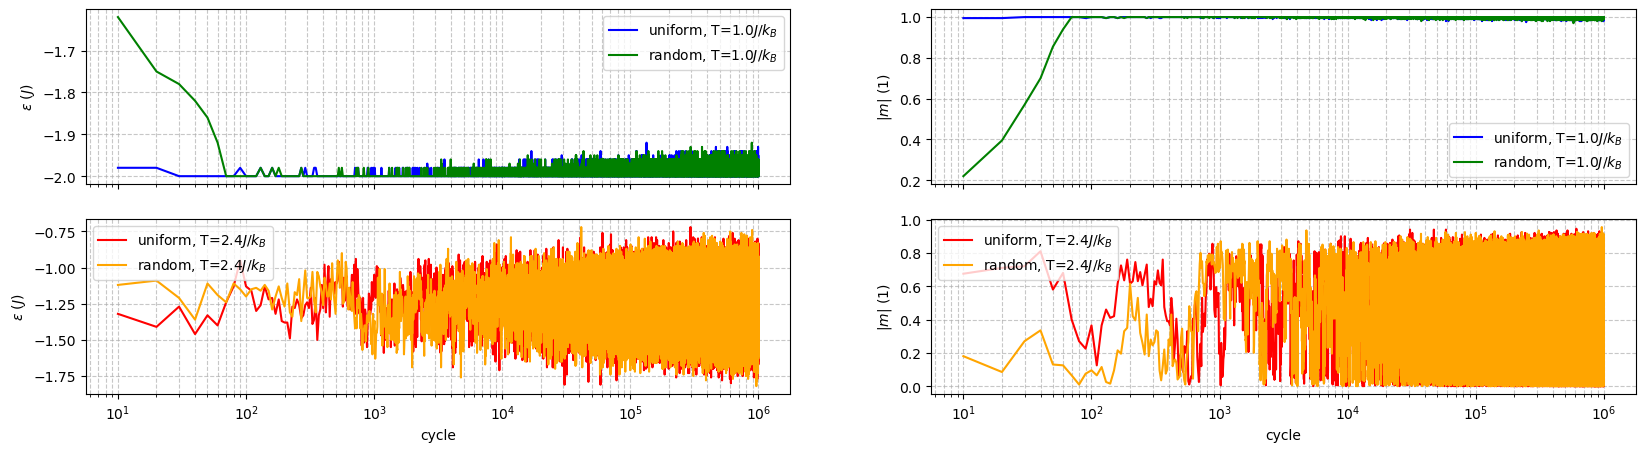
\includegraphics[width=0.95\linewidth]{Project 4/figures/p5_equilibration_rawvalues.png}
    \caption{The $\epsilon$ and $|m|$ values as a function of Monte Carlo cycles using a $20\times 20$ Ising model. The x-axis is a log axis. Uniform refers to a simulation where all samples point up at , while random refers to a random initialization of each dipole. }
    \label{fig:p4_p5_equilibration}
\end{figure*}

We study the equilibration time of the model using a $20\times 20$ Ising model. Figure \ref{fig:p4_p5_equilibration} shows the values of $\epsilon$ and $|m|$ as a function of the Monte Carlo cycles. The results are shown on a log x-axis. The temperature is $T=1~J/k_B < T_c$ and $T=2.4~J/k_B > T_c$ for the upper and lower panels, respectively. Uniform and random refer to the initialization method of the lattice as described in Section \ref{sec:p4_implementation}. 


The results show that there is a clear temperature dependency in how the energy and magnetization evolve through the cycles. For the low temperature $T=1~J/k_B$, the system converges quicly to a stationary state, only deviating from time to time as seen in the earlier cycles of the simulation. This can be understood as a result of the Metropolis criterion. For the low temperature, the dipoles want to align. Therefor, a flip of a dipole will yield a high, positive change in energy (ref Table \ref{tab:p4_delE}). The result is that the flip is left to the weather or not the relative Boltzmann factor $e^{-\beta \Delta E}$ is smaller than $r\sim U[0,1]$. This yields a very low probability of dipole flipping for lower temperatures. This concept also explains why the uniformly initated lattice reaches equilibrium quicker than the randomly generated one for low temperatures, as shown using the expectation values in Figure \ref{fig:p4_appb_p5_expectation_convergence}. Further Figure \ref{fig:p4_appb_p5_expectation_convergence} shows two important aspects of the Ising model. Firstly, it shows how higher temperatures increase the energy, but also that the magnitude of magnetization is substantially decreased when surpassing the Curie temperature. Secondly, it shows that the convergence is much smoother for lower temperatures, i.e., there is more oscillation around an equilibrium for higher temperatures, as backed by looking at $T=2.4~J/k_B$ in Figure \ref{fig:p4_p5_equilibration}. Lastly, we can see that the convergence rate is only marginally faster for a uniformly initalized lattice compared to the randomly initialized. This is because at $T>T_c$ the alignment of dipoles is not generally favored as discussed in the theory.

Using Figure \ref{fig:p4_p5_equilibration} and \ref{fig:p4_appb_p5_expectation_convergence} we see that the equilibration time is somewhere in the range of $10^{4}-10^{5}$ Monte Carlo cycles. At this, the system is producing oscillations of $\epsilon$ and $|m|$ at fairly constant magnitude, and their expectation values are ''settled``, also for temperatures above the Curie temperature.


\subsection{Approximating the probability distribution of energy}

Knowing the equilibration time we can now use cycles after this point to estimate the probability density function of the energy. Figure \ref{fig:p4_p6pdf} shows the relative or \textit{density}-based histogram for the $T=1~J/k_B$ and $T=2.4~J/k_B$. Note that log y-axis.

\begin{figure}[h!]
    \centering
    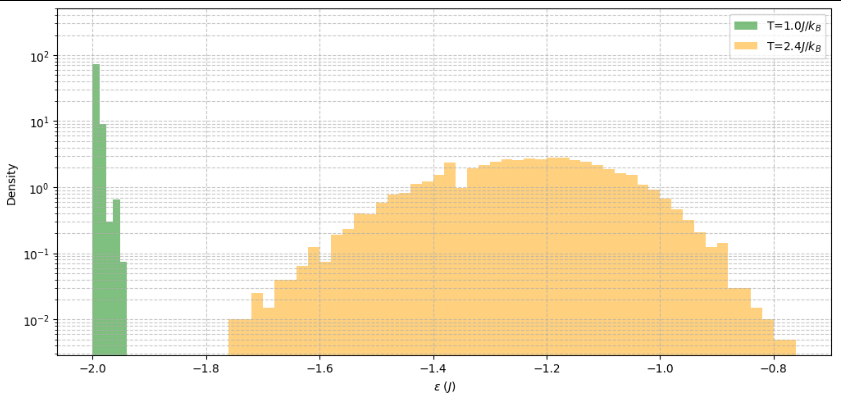
\includegraphics[width=0.8\linewidth]{Project 4/figures/p6_pdfeps.png}
    \caption{The density histograms of energy. Samples are taken after equilibrating the model.}
    \label{fig:p4_p6pdf}
\end{figure}

The results are consistent with previous findings indicating that exceeding $T_c$ significantly increases both the mean energy and also the spread of samples. Estimated based on the samples shown in the figure, the variance is $1.89*10^{-5}$ and $2.01*10^{-2}$ for low and high temperatures, respectively.

\subsection{Phase transitions}

To study the phase transition, we investigate the relation between lattice size (L), temperature (T), and the output variables. We do this by running simulations for $L\in\{40,60,80,100\}$ as well as temperatures $T\in[2.1, 2.4]~J/k_B$, which is the region encompassing the analytical critical value of $\approx 2.269~J/k_B$ from equation \eqref{eq:p4_critical_temp}. Figures \ref{fig:p8_eps}, \ref{fig:p8_cv}, \ref{fig:p8_mabs} and \ref{fig:p8_chi} show the relation between $\mathbb{E}[\epsilon]$, $C_V/N$, $\mathbb{E}[|m|]$, $\chi/N$ and temperature, respectively. In addition, they show how the expectation values around the phase transition depend on L.

\begin{figure}[h!]
    \centering
    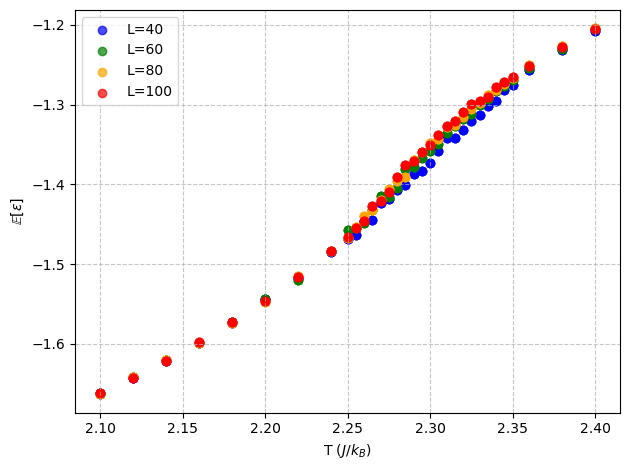
\includegraphics[width=0.8\linewidth]{Project 4/figures/p8_eps.png}
    \caption{The expectation value of the energy per dipole $\epsilon$ as a function of temperature $T$ for Ising models of different lattice sizes. We display the relation around the analytical Curie temperature to study phase transitions.}
    \label{fig:p8_eps}
\end{figure}
\begin{figure}[h!]
    \centering
    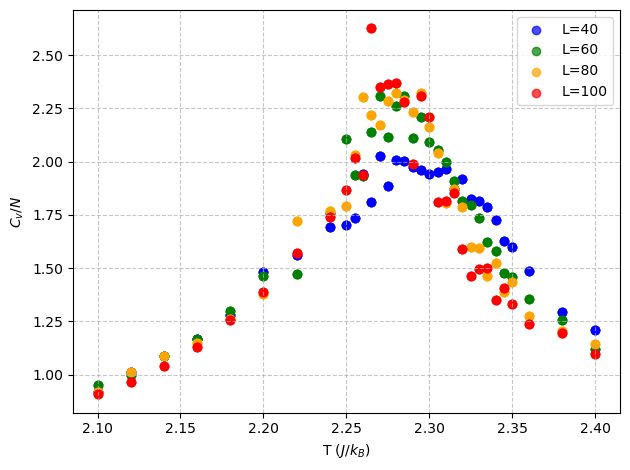
\includegraphics[width=0.8\linewidth]{Project 4/figures/p8_cv.png}
    \caption{The heat capacity per dipole $C_V/N$ as a function of temperature $T$ for Ising models of different lattice sizes. We display the relation around the analytical Curie temperature to study phase transitions.}
    \label{fig:p8_cv}
\end{figure}
\begin{figure}[h!]
    \centering
    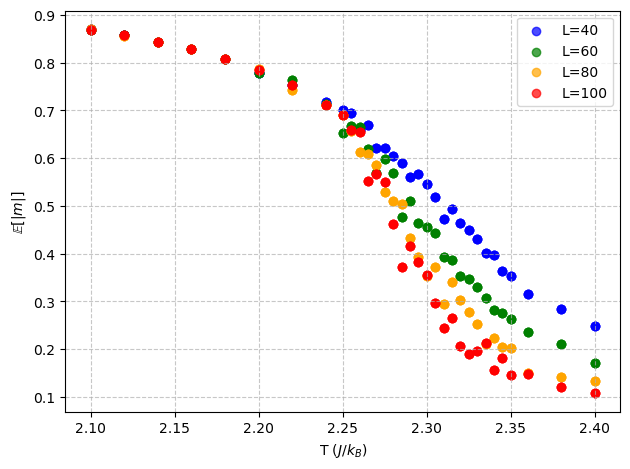
\includegraphics[width=0.8\linewidth]{Project 4/figures/p8_mabs.png}
    \caption{The expectation value of the absolute value of magnetization per dipole $|m|$ as a function of temperature $T$ for Ising models of different lattice sizes. We display the relation around the analytical Curie temperature to study phase transitions.}
    \label{fig:p8_mabs}
\end{figure}
\begin{figure}[h!]
    \centering
    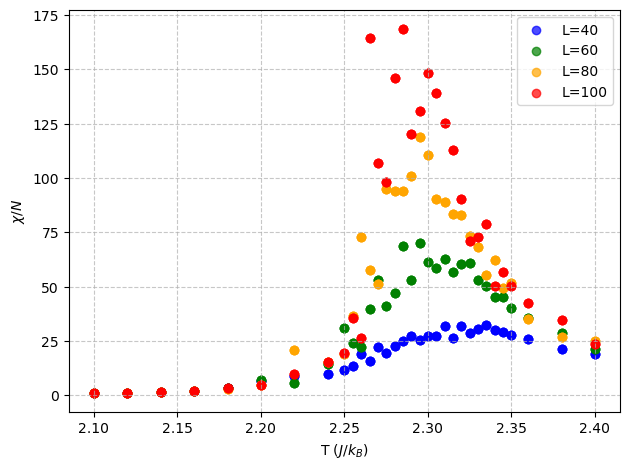
\includegraphics[width=0.8\linewidth]{Project 4/figures/p8_chi.png}
    \caption{The susceptibility per dipole $\chi/N$as a function of temperature $T$ for Ising models of different lattice sizes. We display the relation around the analytical Curie temperature to study phase transitions.}
    \label{fig:p8_chi}
\end{figure}

In Figures \ref{fig:p8_cv} and \ref{fig:p8_chi}, we see how the normalized per dipole heat capacity and magnetic susceptibility depend on temperature. Following from equations \eqref{eq:p4cv1} and \eqref{eq:p4chi1}, we know that for $T$ close to $T_c$, the $C_V$ and $\chi$ values should diverge. Since we are doing a numerical analysis (and the resolution is coarse (ref Section \ref{sec:future_work}), we will not observe this. The phase transition is rather observed as a peak for both of these variables. In accordance with equations \eqref{eq:p4cv2} and \eqref{eq:p4chi2}, the magnitude of the peak is proportional to the lattice, with (in general) larger values for larger L's. Further, we observe from Figure \ref{fig:p8_mabs} that there is a phase transition for the magnetic domain as temperatures rise; that is, the magnetization indeed is rapidly decreased. We also see that the convergence is faster for larger models, indicating that a large model is more in line with the theory for real materials. There is no similar phase transition for the energy in the model. This is seen from Figure \ref{fig:p8_eps}, where there is only a small divergence between lattice sizes, with larger ones increasing faster. This can be explained by the higher heat capacity per dipole for larger models, as seen in Figure \ref{fig:p8_cv}. For temperature values on either side of the phase transition, there are very large differences between lattice sizes.

To estimate the Curie temperature for $L=\infty$ and benchmark the simulations against the analytical results of equation \eqref{eq:p4_critical_temp}, we start by estimating $T_c(L)$. The estimation is done by picking the largest value of $\chi/N$ for each $L$. Further, we fit a regression line using \textit{scipy.stats.linregress}. Using this, we can use the intercept as our prediction of $T_c(L=\infty)$ because $1/L \to 0$ as $L\to \infty$. The results shown in Figure \ref{fig:p4regression_predictedTc} show the temperature values used for the regression fit as well as the regression predicted value for $L=\infty$.

\begin{figure}[h!]
    \centering
    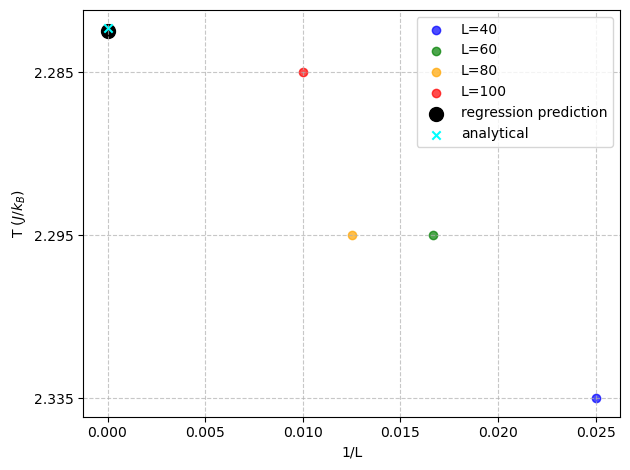
\includegraphics[width=0.9\linewidth]{Project 4/figures/p9_predictedTc.png}
    \caption{The regression predicted $T_c$ value for a $L=\infty$ Ising model. The regression is based on $T_c(L)$ values estimated by taking the max value of $\frac{\chi}{n}(L)$.}
    \label{fig:p4regression_predictedTc}
\end{figure}

Comparing with the analytical results of $T_c=2.269~J/k_B$, the regression estimate based on $\hat{T}_c(L)$ values is fairly close at $\hat{T}_c=2.251~J/k_B$. The goodness of fit, that is, the $R^{2}$ value for the regression line, is $0.96$; however, investigations of the validity of this extrapolation should be done before concluding further.

\subsection{Future work and improvements}\label{sec:future_work}

For this project, we were unable to create a parallelized code where the computational overhead did not outweigh the benefit. Because of this, the temperature resolution when investigating the critical temperature is very coarse. This makes the identification of the ''true`` $T_c(L)$ difficult, thus effecting the resulting estimate of $T_c(\infty)$. Therefore, for future work, a re-implementation with parallelization should be done. This will allow for a more effective sampling and more robust results.

\end{document}
